\documentclass{standalone}

\usepackage{graphicx}
\usepackage{stackengine}
\usepackage{tikz}
\usepackage{amssymb}
\usepackage{mathdots}

\usetikzlibrary{positioning}
\usetikzlibrary{shapes.geometric}
\usetikzlibrary{calc}
\usetikzlibrary{decorations.pathreplacing}
%% \usetikzlibrary{arrows}
\usetikzlibrary{arrows.meta}
%% \tikzset{%
%%   strongT/.tip={Triangle},/.style={line width=12mm}
%% }
\newcommand\vcdots{\;\stackMath\stackinset{c}{0pt}{c}{0.6ex}{\vdots}{\vphantom{-}}\;}
%% \setstackgap{S}{inter-item stackgap}
%% \setstackgap{L}{1.2em}

\begin{document}

\tikzset{every picture/.style={line width=0.9pt}}

%% \begin{figure}[p] % remove when finished
\begin{tikzpicture}[
networknode/.style={regular polygon,regular polygon sides=4, draw=black, fill=none, line width=0.8mm, inner sep=-60pt},
vectornode/.style={rectangle, draw=black, fill=none, },
internode/.style={rectangle, draw=black, fill=none, thick},
imagenode/.style={rectangle, draw=none, fill=none},
>={Triangle[width=4mm,length=2.9mm]},->
]

%Nodes
% What sorta style should the text have? Blue ass well?
% mention a cnn somewhere
% also see https://www.researchgate.net/figure/The-high-level-concept-of-an-extended-variational-autoencoder-adopted-for_fig8_317486066
% http://bjlkeng.github.io/images/variational_autoencoder2.png
\node[imagenode] (input) [] [label=below:{$X$}]{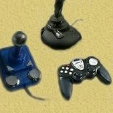
\includegraphics[width=0.052\textwidth]{in.png}};
\node[networknode] (encoder) [right=of input][text width=10.1cm, align=center, label=below:{\mbox{$Q(z|X)$}}][label=above:{convolutions}]
     {\textbf{Encoder Network}};
\node[right=3.0cm of encoder] (dummy) {}; 
\node[internode] (mean) [below=1.4of dummy] {$\mu(X)$};
\node[internode] (std) [above=1.4of dummy] {$\Sigma(X)$};
\setstackgap{L}{0.9em}
\node[vectornode] (latent) [right=3.0cm of dummy] {\Vectorstack{{z_1} \textbf{.} \textbf{.} \textbf{.}  {z_n}}};
%% \node[vectornode] (latent) [right=3.0cm of dummy] {\Vectorstack{{z_1} {\large; \vdots}  {z_n}}};
\node[networknode] (decoder) [right=2.0cm of latent][text width=10.1cm, align=center, label=below:{\mbox{$P(X|z)$}}][label=above:{transposed convolutions}]{\textbf{Decoder Network}};
\node[imagenode] (output) [right=of decoder][label=below:$\widetilde{X}$] {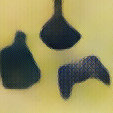
\includegraphics[width=0.052\textwidth]{out.png}};

%Lines
%% \draw[-strongT, line width=0.35mm] (input.east) -- (encoder.west);
\draw[->] ($(input.east) + (-0.3, 0)$) -- (encoder.west);
%% \draw (encoder.south) node[label=below:$b_1$,draw]{}
\draw[->] ($(encoder.east)+(0,0.3)$) |- ++(.5,0.0) -- ++(0, 0.9) |- (std.west);
\draw[->] ($(encoder.east)+(0,-0.3)$) |- ++(.5,-0.0) -- ++(0, -0.9) |- (mean.west);
\draw[->] (mean.east) |- ++(.5,-0.0) -- ++(0, 0.0) |- ($(latent.west)+(0, -0.3)$);
\draw[->] (std.east) |- ++(.5,-0.0) -- ++(0, -0.0) |- ($(latent.west)+(0, 0.3)$);
\draw[->] (latent.east) -- (decoder.west);
\draw[->] (decoder.east) -- ($(output.west) + (0.3,0)$);
\tikzset{>={Triangle[width=0.001mm,length=0.01mm]},->}
\draw[decorate,decoration={brace, amplitude=13pt}] (latent.east |- 0, -3.65) --
        node[below, yshift=-5.3mm]{sample $z \thicksim \mathcal{N}(\mu(X), \Sigma(X))$} (mean.west |- 0, -3.65); 
%% \draw[->] (decoder.west) .. controls +(down:7mm) and +(right:7mm) .. (lowercircle.east);
%% \draw[->] (decoder.west) 

\end{tikzpicture}
%% \end{figure}

\end{document}
